\documentclass{amsart}

\usepackage[english]{babel}
\usepackage[utf8]{inputenc}
\usepackage{graphicx}
\usepackage{mathtools}
\usepackage{amsthm}
\usepackage{amsfonts}
\usepackage{hyperref}
\usepackage[singlelinecheck=false]{caption}
\usepackage[backend=biber,url=true,doi=true,eprint=false,style=alphabetic]{biblatex}
\usepackage{enumitem}
\usepackage[justification=centering]{caption}
\usepackage{indentfirst}
\usepackage{algorithm}
\usepackage{algpseudocode}

\addbibresource{references.bib}

\makeatletter
\def\subsection{\@startsection{subsection}{3}%
  \z@{.5\linespacing\@plus.7\linespacing}{.1\linespacing}%
  {\normalfont\itshape}}
\makeatother

\DeclareMathOperator*{\argmin}{arg\,min}
\DeclareMathOperator*{\argmax}{arg\,max}

\newcommand\defeq{\mathrel{\overset{\makebox[0pt]{\mbox{\normalfont\tiny\sffamily def}}}{=}}}

\algrenewcommand\algorithmicrequire{\textbf{Input}}
\algrenewcommand\algorithmicensure{\textbf{Output}}

\captionsetup[table]{labelsep=space}

\theoremstyle{plain}

\newtheorem*{definition}{Definition}
\newtheorem{theorem}{Theorem}
\newtheorem{proposition}{Proposition}

\newcommand{\set}[1]{\mathcal{#1}}
\newcommand{\pr}{\mathbb{P}}
\renewcommand{\implies}{\Rightarrow}

\setlength{\parskip}{1em}

\title[]{2. Bayesian Networks}
\author[]{Renato Lui Geh\\NUSP\@: 8536030}

\begin{document}

\begin{abstract}
  In this document we present general, basic notions of bayesian networks. We present a brief
  introduction to graph theory, where we show a few elementary definitions and properties of an
  acyclic directed graph. We introduce the concept of factors and how to perform the product of two
  factors and the summing-out of a variable. We then focus on Bayesian networks, presenting main
  definitions and properties related to the subject. Important concepts such as Markov's Property,
  factoring of bayesian networks and barren nodes are formally defined. We then show common
  bayesian structures, namely Naive Bayes, Bipartite Bayesian Networks and Polytrees.
  \vspace*{-2.5em}
\end{abstract}

\maketitle

\section{Basic Notions of Graph Theory}

A graph $G$ can be represented as an ordered pair $(V,E)$, where $V$ is the set of vertices (or
nodes) and $E$ is the set of edges (or arcs). An edge $e\in E$ has an origin node $i\in V$ and a
destination node $j\in V$. This edge can be represented as a pair $(i,j)$. In an undirected graph,
$(i,j)=(j,i)$. A path from a node $n_i$ to another $n_j$ is a sequence of distinct nodes and
distinct edges that begin and end with vertices. A connected graph is a graph where every node in
$V$ can be reached by a path. An acyclic graph is a graph where there must not exist an infinite
path.

Let $(x,y)$ be a pair of nodes in $V$, and $V$ is the set of nodes in an acyclic directed graph
$G=(V,E)$. Then $x$ is a parent of $y$ iff there exists an edge $x\to y$ in $E$, where $\to$
denotes a directed edge from node $x$ to node $y$. In this case, $y$ is a child of $x$. We will
denote the set of parents of an arbitrary node $x$ as $Pa(x)$. Similarly, the set of children of
$x$ is $Ch(x)$. In an acyclic directed graph (DAG), the indegree of a node $x$ is the number of
parents of $x$, that is $deg^-(x)=|Pa(x)|$. Equivalently, the number of children of $x$ is called
the outdegree and is denoted by $deg^+(x)=|Ch(x)|$.

In this report, when we refer to a graph we implicitly define it as a DAG, unless we explicitly
specify it as otherwise. The ancestrals of a node $x$ is the set $An(x)=\{Y:(y,x)\in E$ or $(y,z)
\in E$ and $z\in An(x)\}$, that is, $An(x)$ is a set of all nodes $y\in An(x)$ where there exists a
path from $y$ to $x$. The descendants of $x$ is the set $De(x)$ of all nodes where there exists a
path from a descendant node to $x$. The non-descendants of $x$, denoted by $Nd(x)$ is the set of
nodes that are not in $De$. If a graph $G=(V,E)$ obeys the rule $|E|=O(n)$, where $n=|V|$, then it
is said to be sparse.

A sequence of nodes $x_1,\ldots,x_n$ is a topological ordering iff the graph is acyclic and if it
obeys $i<j \implies i\in De(x_j)$.

\section{Factors}

Consider functions $f$ and $g$. Let $\nu$ be a valuation such that $\nu : x\mapsto dom(x)$. Then we
define $f(x)\nu$ as a function where the set $x$ of variables is instantiated so that it satisfies
$\nu$. For instance, let $\nu(A)=1$ and $\nu(B)=0$. Then:


\begin{equation*}
  f(A,B)\nu \equiv f(A=1,B=0)
\end{equation*}

The product of two functions is then defined as:

\begin{align*}
  &f(x)g(y)=h(x,y)\\
  &h(x,y)\nu=f(x)\nu g(y)\nu
\end{align*}

We denote $\sigma(f)$ as the scope of function $f$. Note that $\sigma(h)=\sigma(f)\cup\sigma(g)$.
The summing-out of a variable eliminates a variable $x$ from the scope of a function $f$.

\begin{align*}
  &y \in \mathbf{x} \implies \sum_y f(\mathbf{x}) = f(\mathbf{x})\nu + \sum_{\nu':\nu(A)\neq
  \nu'(A)} f(\mathbf{x})\nu'\\
  &y \neg\in \mathbf{x} \implies \sum_y f(\mathbf{x}) = f(\mathbf{x})
\end{align*}

If we assume that the product and variable elimination operations obey the associativity law (i.e.
$f(x)g(y)=g(x)f(y)$) and are also comutative (i.e. $f(x)[g(y)h(z)]=[f(x)g(y)]h(z)$), we then have
that:

\begin{equation*}
  \sum_A\sum_B f(x) = \sum_B\sum_A f(x) = \sum_{A,B} f(x)
\end{equation*}

When a variable is not present in the scope of a function, we may take the function out of the
summation. For instance, consider the functions $f$ and $g$, with scopes $\sigma(f)=\{A,B\}$ and
$\sigma(g)=\{C\}$. Then we have the distributive property:

\begin{equation*}
  \sum_{A} f(x)g(x) = g(x) \sum_{A} f(x)
\end{equation*}

This allows for fewer operations, since product of functions increases the number of elements,
which, in this case, could result in redundant operations. When we deal with distribution of
probabilities, we may refer to these functions as factors. A factor maps the instantiations of the
variables to their respective probabilities. Conditional probability tables (CPTs) are one form of
factor, as are joint distributions. We can see the scope of a function $\sigma(f)$ as the scope of
the distribution. When we perform a product of functions we are actually combining all possible
values of two distributions into one table. The summing-out, or variable elimination, of a factor
sums out all probabilities of a variable.

\section{Markov's Property}

Consider a probability distribution $\pr$. Then $\pr$ satisfies Markov's Property (MP) wrt a DAG
$G=(V,E)$ if:

\begin{align*}
  x\in V &\implies x \perp Nd(x)|Pa(x)\\
         &\implies x \perp Nd(x)\setminus Pa(x) | Pa(x)
\end{align*}

That is, for all node $x$ in DAG $G$, $x$ is independent of the non-descendants non-parents given
its parents. We will denote independence through a function $I$. We say that a set of nodes
$\mathbf{x}$ is independent of a set of nodes $\mathbf{y}$ given set $\mathbf{z}$ if $I(\mathbf{x},
\mathbf{z},\mathbf{y})$. Let $\mathbf{x}$ be the set of nodes where $\forall x \in \mathbf{x}$,
$Pa(x)=\emptyset$, then we have that $I(\mathbf{x}, \emptyset, Nd(\mathbf{x}))$ and therefore we
can say that all root nodes are marginally independent from their non-descendants.

\section{Bayesian Networks}

A Bayesian Network (BN) is composed of three elements $(G, \mathcal{L}, \pr)$, where:

\begin{itemize}
  \item $G$ is a DAG with nodes and edges $(V,E)$
  \item $\mathcal{L}$ is a propositional language with variables $V$
  \item $\pr$ is a probability function that satisfies MP wrt $G$
\end{itemize}

Alternatively, a BN can be seen as a directed acylic graph where nodes are related to variables in
the probability distribution the network represents, with each variable associated with a
conditional probability table (CPT) that enumerates all probabilities of a variable given its
dependencies. In fact, from Markov's Property, we have that, since every node is independent of its
non-descendants non-parents, then applying the chain rule on the full joint distribution, we have
that:

\begin{theorem} Factorization Theorem~\label{factor-thm}\\
  Let $\mathcal{N}$ be a bayesian network with variables $X_1,\ldots,X_n$, then we have that:
  \begin{equation*}
    \pr(X_1,\ldots,X_n) = \prod_{X_i} \pr(X_i|Pa(X_i))
  \end{equation*}
\end{theorem}

In fact, a bayesian network is a bayesian network iff it satisfies the Factorization Theorem.
Furthermore, the Factorization Theorem is valid iff the BN satisfies Markov's Property. As we can
see from Theorem~\ref{factor-thm}, the full joint distribution can be found by the product of all
conditional probabilities of a variable given its parents. These conditional probabilities are
called conditional probability tables (CPTs), and each variable has one associated with it.

\begin{table}[h]
  \centering{\captionsetup{justification=centering}
    \begin{tabular}{c c | c}
      $A$ & $B$ & $\Theta_{B|A}$\\
      \hline
      true & true & $0.2$\\
      true & false & $0.4$\\
      false & true & $0.8$\\
      false & false & $0.6$\\
    \end{tabular}
    \caption{A CPT of variable $B$ with $Pa(B)=\{A\}$.}\label{cpt-1}
  }
\end{table}

We call the conditional probabilities $\Theta_{X_i|Pa(X_i)}$ the parameters (or the CPT of variable
$X_i$) of the bayesian network. Each probability $\theta_{X_i=x_i|Pa(X_i)}$ is a parameter and must
obey $\sum_{x_i} \theta_{X_i=x_i|Pa(X_i)} = 1$. For instance, $\theta_{A=true|B=true}+
\theta_{A=false,B=true}=\theta_{A=true|B=false}+\theta_{A=false|B=false}=1$, on the CPT of
Figure~\ref{cpt-1}. A network parameter is compatible with an instanciation $\mathbf{z}$ when all
the values from the instantiation are the same as in the network parameter. That is, the parameter
$\theta_{\mathbf{x}|\mathbf{u}}$ is compatible with $\mathbf{z}$ iff $\mathbf{x}\cup\mathbf{u}
\subseteq\mathbf{z}$. We will denote this compatibility as $\theta_{\mathbf{x}|\mathbf{u}}\sim z$.

\section{Barren Nodes}

Let $X$ be a node and $S$ a set of nodes. $X$ is barren wrt $S$ if $\{X\}\cup De(X)\cap
S=\emptyset$.

\begin{figure}[h]
  \captionsetup{justification=centering}
  \centering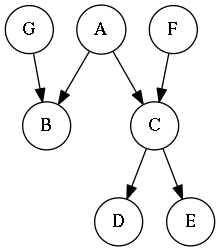
\includegraphics[scale=0.5]{graphs/barren.png}
  \caption{$C$ is barren wrt $S$ when $S=\{A,B,G\}$.}
\end{figure}

Consider a probability distribution $Pr_G$ that satisfies Markov's Property wrt the graph $G$. Then
if $\mathcal{B}$ is the set of barren nodes wrt the set $S$ and $H=(V-\mathcal{B},E')$ the
resulting graph after the removal of every node in $\mathcal{B}$ and their respective edges from
$G$, we can afirm that $Pr_G(S)=Pr_H(S)$, where $Pr_H(V-\mathcal{B})=\prod_{X\in V-\mathcal{B}}
Pr_G(X|Pa(X))$. That is, removing all barren nodes from the graph given a set $S$ is guaranteed for
the value of queries to remain the same as long as the query does not reference any node in
$\mathcal{B}$. This decreases the computational complexity when the graph is too big, since we may
shorten it into a simpler, easier graph to compute queries on.

\section{Exact Inference on Bayesian Networks}

Exact inference on bayesian network is computationally intractable, since it is exponential on the
number of elements in the distribution. In this section we see how to perform queries through
elimination of variable, a technique to compute exact inference on bayesian networks by summing-out
variables and multiplying factors.

\subsection{Marginals}

We call evidence an instantiation of variables. A marginal is the probability of evidence of a
subset of values of variables. That is, let $\mathbf{X}=\{X_1,\ldots,X_n\}$ be the set of variables
in the distribution, then the prior marginal distribution of $m$ variables where $m\leq n$ is:

\begin{equation*}
  \pr(X_1,\ldots,X_m)=\sum_{x_{m+1},\ldots,x_n} \pr(X_1,\ldots,X_n)
\end{equation*}

That is, the prior marginal distribution is the distribution summed-out over the variables that are
not present in the prior marginal's scope. Similarly, the posterior marginal distribution is
computed by summing-out the variables not present in the posterior marginal's scope:

\begin{equation*}
  \pr(X_1,\ldots,X_m|\mathbf{e})=\sum_{x_{m+1},\ldots,x_n} \pr(X_1,\ldots,X_n)
\end{equation*}

\subsection{Computing Queries}

To compute the probability of an evidence in a bayesian network, we must first compute the full
joint distribution to then compute the marginal. Once we have the full joint distribution we may
sum-out the variables not present in the scope of the evidence, acquiring the probability of the
marginal. To compute the full joint distribution we must recall Theorem~\ref{factor-thm}:

\begin{equation*}
  \pr(X_1,\ldots,X_n) = \prod_{X_i\in \mathbf{X}} \pr(X_i|Pa(X_i))
\end{equation*}

Note that in order to compute the full joint distribution we have to compute the product of all
factors (i.e. CPTs). To alleviate the computational complexity we may apply the distributive law
over the factors in this product. Once we have the full joint distribution, we may compute the
marginals given the evidence.

\begin{equation*}
  \pr(\mathbf{e}=\{X_1=x_1,\ldots,X_m=x_m\}) = \sum_{x_{m+1},\ldots,x_n} \pr(x_1,\ldots,x_n)
\end{equation*}

To compute a posterior probability, we compute the probability of evidence and then apply the
conditional probability definition. Let $\mathcal{X}$ be a set of instantiations of query
variables, $\mathbf{X}$ the set of all variables in the bayesian network and $\mathbf{e}$ be the
set of evidence values. Then:

\begin{equation*}
  \pr(\mathcal{X}|\mathbf{e})=\frac{\pr(\mathcal{X},\mathbf{e})}{\pr(\mathbf{e})}=
  \frac{\sum_{\mathbf{X}\setminus(\mathcal{X}\cap\mathbf{e})} \pr(\mathbf{X})}{\sum_{\mathbf{X}
  \setminus\mathbf{e}} \pr(\mathbf{X})}
\end{equation*}

Note that this requires the summing-out of a product over all variables. This is evidently
exponential over the number of terms in the probability distribution.

\section{Common Structures}

There are structures that are commonly used due to their simplicity or specific properties. Here
we show three of such structures: Trees, Naive Bayes, Bipartite Bayesian Networks and Polytrees.

\subsection{Tree}

A tree-shaped bayesian network is a BN where each node has at most one parent. Since we have no
guarantees in relation to connectivity, this allows disconnected graphs. A disconnected graph is
a graph where, when taking the underlying undirected graph, there exists at least one pair of nodes
which have no path between them.

\begin{figure}[h]
  \captionsetup{justification=centering}
  \centering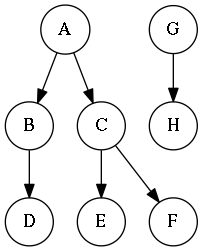
\includegraphics[scale=0.5]{graphs/tree.png}
  \caption{A tree with root nodes $A$ and $G$. The graph with root $A$ is disconnected from the
  graph with root $G$, since there is no connecting path betweem the two graphs.}
\end{figure}

\begin{proposition} Exercise 1\\
  The number of probability values in a tree-shaped Bayesian Network with discrete variables is
  $\mathcal{O}((n-1)p^2)$, where $p$ is the greatest number of possible values a variable may take.
\end{proposition}

\begin{proof}
  In a tree-shaped Bayesian network a node may have up to one parent node. The number of
  probability values in a root node is $p_i$, where $p_i$ is the number of values a variable $i$
  may take. An intermediary node may have $p_j^2$ probability values, since it may only have one
  parent by definition. Consider $p$ the greatest number of possible values any variable in the
  bayesian network may take. Then $\mathcal{O}(p)\geq\mathcal{O}(p_i)$ for any $i$. Since
  $\mathcal{O}(p^2)\geq\mathcal{O}(p)$, a tree-shaped bayesian network must have, at maximum,
  $(n-1)p^2+p=\mathcal{O}((n-1)p^2)$ probability values. Note that an $(n-1)p^2+p$ tree-shaped
  bayesian network is a Naive Bayes.
\end{proof}

\subsection{Naive Bayes}

A Naive Bayes is composed of one parent, or class, and multiple children, or attributes. This
structure is commonly used for classification, as it describes features as children and possible
classifications as the root node. One can easily see a Naive Bayes is a tree where all non-root
nodes are children of the root node.

\begin{figure}[h]
  \captionsetup{justification=centering}
  \centering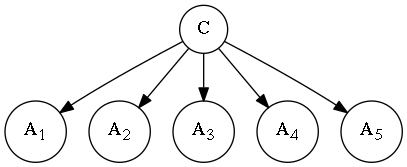
\includegraphics[scale=0.5]{graphs/naive_bayes.png}
  \caption{A Naive Bayes with class $C$ and attributes $A_1,\ldots,A_5$.}
\end{figure}

\begin{proposition} Exercise 3\\
  Let $\mathcal{N}$ be a Naive Bayes model with node $C$ as root node and $A_1,\ldots,A_n$ as
  children. Then for every $A_i$, $A_i \perp A_j$, $i\neq j$.
\end{proposition}

\begin{proof}
  Let $\mathbf{X}$ be the set of all variables in $\mathcal{N}$. From Markov's Property, we have
  that:

  \begin{equation*}
    A_i \perp Nd(A_i)\setminus Pa(A_i) | Pa(A_i)
  \end{equation*}

  But $Nd(A_i)\setminus Pa(A_i)=Ch(C)\setminus \{A_i\}$. Therefore $A_i \perp Ch(C)\setminus
  \{A_i\}|Pa(A_i)$.
\end{proof}

\subsection{Bipartite}

A bipartite bayesian network is a bayesian network whose graph can be partitioned into two sets of
nodes. Every node in the first set has at least one edge to another node in the other set, has
no edge to a node to another element on its own set and no element in the second set has an edge
to an element in the first set. That is, let $P_1$ and $P_2$ be two sets, $P_1\cap P_2=\emptyset$
and $P_1\cup P_2=V$, where $V$ is the set of nodes in the bayesian network $\mathcal{N}$. Then for
all $e\in E$, where $E$ is the set of edges in $G$, $e$ is of the form $(v_i^1,v_j^2)$, where
$v_i^1$ is a node in $P_1$ and $v_j^2$ is a node in $P_2$.

\begin{figure}[h]
  \captionsetup{justification=centering}
  \centering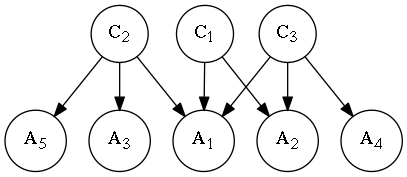
\includegraphics[scale=0.5]{graphs/bipartite.png}
  \caption{A Bipartite Bayesian Network with partitions $P_1=\{C_1,C_2,C_3\}$ and $P_2=\{A_1,A_2,
  A_3,A_4,A_5\}$.}
\end{figure}

\begin{proposition} Exercise 2\\
  The number of probability values in a bipartite bayesian network with $m$ root variables and $n$
  leaves is $\mathcal{O}(np^m+mq)$, where $p$ is the number of values a leaf may take and $q$ when
  it is a root node.
\end{proposition}

\begin{proof}
  For
\end{proof}

\newpage

\printbibliography[]

\end{document}
